\documentclass[11pt, twoside, reqno]{book}
\usepackage{amssymb, amsthm, amsmath, amsfonts}
\usepackage{multicol}
\usepackage{titlesec}
\usepackage{graphicx}
\usepackage{amsrefs}
\usepackage{color}
\usepackage{hyperref}
\usepackage{verbatim}
\usepackage{calc}
\usepackage{fancyhdr}
\usepackage{tcolorbox}
\tcbuselibrary{skins,breakable,raster}
\usepackage[toc,page]{appendix}
\appendixpageoff

\usepackage{prftree}

\usepackage{bardtex}
\styleoption{seniorproject}

\iftrue
\makeatletter
\renewcommand{\chaptermark}[1]{%
  \markboth{%
    \chaptername\ \thechapter.\ \ #1
  }{}%
}

\renewcommand{\sectionmark}[1]{\markright{\thesection.\ \ #1}}

\fancyhead{} % Clears the standard fancy style
\fancyhead[L]{\scshape \nouppercase{\rightmark}}
\fancyhead[R]{\scshape \nouppercase{\leftmark}}

\renewcommand\tableofcontents{%
    \if@twocolumn
      \@restonecoltrue\onecolumn
    \else
      \@restonecolfalse
    \fi
    \chapter*{\contentsname
        \@mkboth{%
           \contentsname}{\contentsname}}%
    \@starttoc{toc}%
    \if@restonecol\twocolumn\fi
    }

\makeatother
\fi

\iftrue
\usepackage{unicode-math}
\setmainfont{Libertinus Serif}
\setsansfont[Scale=MatchUppercase]{Libertinus Sans}
\setmathfont{Libertinus Math}
%\setcodefont{Inconsolata}
\else
\ifxetex
\RequirePackage[libertine]{newtxmath}
\RequirePackage[tt=false]{libertine}
\setmonofont[StylisticSet=3]{inconsolata}
\else
\ifluatex
\RequirePackage[libertine]{newtxmath}
\RequirePackage[tt=false]{libertine}
\setmonofont[StylisticSet=3]{inconsolata}
\else
\RequirePackage[tt=false, type1=true]{libertine}
\RequirePackage[varqu]{zi4}
\RequirePackage[libertine]{newtxmath}
\fi
\fi
\fi

%Your macros, if you have any.
\DeclareMathOperator{\imax}{imax}
\DeclareMathOperator{\ifop}{if}

\begin{document}

\renewcommand{\contentsname}{Contents}
\fancyhead[LE]{\textit{\nouppercase{\leftmark}}}
\fancyhead[RO]{\textit{\nouppercase{\rightmark}}}

%For senior projects:
\titlepg{The Algebra of Type Unification}{Verity James Scheel}
    {December}{2021}

\abstr

Type unification takes type inference a step further by allowing non-local flow of information. By exposing the algebraic structure of type unification, we obtain even more flexibility as well as clarity in the implementation. The compositional nature of the algebras involved ensure correctness and reduce arbitrariness: properties such as associativity mean that implementation details of type inference do not leak in error messages, for example. This project is a discovery and implementation of these ideas for the type theory of the Dhall programming language, with implementation in PureScript.


\tableofcontents

%\dedic

%I dedicate this senior project to every person I have ever met in my life.

%\acknowl

%I would like to acknowledge the help I received from every person I have ever met in my life.

\startmain


\intro

The Dhall language is designed to be a straightforward, strongly-typed programming language for specifying and generating configurations for system software.
Despite having sophisticated type system features such as dependent types, its standard is kept simple for ease of implementation.
This is done by requiring each expression to contain extra type information, which is often redundant and tedious for the user to specify.
In particular, lambda abstractions have to specify their input type, even though it can often be figured out from context:
\begin{verbatim}
\(n : Natural) -> n + 1
\end{verbatim}
In this example, the user has to specify that the variable \verb`n` has type \verb`Natural`, even though that is the only type that makes the expression typecheck: since the addition operator \verb`+` in Dhall is not overloaded, it can only take two arguments of type \verb`Natural`!
However, because this information requires looking at context (the usage of \verb`n` as an argument to \verb`+`), it is not covered by the current rules of type inference in Dhall.

This project will increase the flexibility of Dhall while still keeping the same philosophy of straightforward type inference rules.
In particular this means adding universe and row polymorphism plus general type unification to the language.
Universes are a technical detail of type theory: they are necessary to allow types to be first-class and they require bookkeeping to ensure the theory remains consistent, but of little interest from a programmer's perspective.
Rows are certainly more interesting from a programmer's point of view: they allow coding to open interfaces, with data addressed by labels, but they have their own challenges in bookkeeping.
In fact, these concepts are already lurking in the existing rules for Dhall, and this project is allowing them to come into their own as concepts represented within the type theory in their own right.

The third idea is the main motivation for this project: general type unification.
In order to allow the programmer to omit more types while writing Dhall, it must be possible to infer what type should have been written in the program, and this is done through unification.
Every omitted type starts off as an unknown type, and the task of unification is to stitch together what partial information is known about a type from its occurrences scattered throughout the program.
But to support the features already in the Dhall language, in this setting of partially unknown types, more or less necessitates the introduction of universe and row variables.
And polymorphism is the natural next step from there: not only will the unknown variables stand for unique-but-unspecified types, but they will actually be able to be instantiated differently across different call sites.

The goal is to maintain bottom-up inference rules in this description of type unification of Dhall.
Traditional unification algorithms in major compilers traverse through program source in a linear fashion, mutating the ``current'' state of unification variables as they go.
This means that information cannot be untangled from the evaluation order the compiler takes, and so the error messages that occur differ depending on program order.
By maintaining the independence of parallel branches of code, the new ideas in this project ensure that errors remain predictable and clear.

The ideas contained in this project should give clearer type errors than both bidirectional typechecking and the usual unification algorithms (which silently mutate unification variables), and it should keep evaluation safe when given partial type information.

% Every senior project should have an introductory chapter that briefly summarizes or previews the content of the whole project.  The introductory chapter, which can be thought of as an expanded version of the abstract, is meant to give the big picture, and should include a discussion of the background to the project, place the project in the context of known results, and provide an informal summary of the main results.  Additionally, the introductory chapter should make clear what in the project is exposition of known results and what is original work.

\section{Type Theory}
\label{TT}

Type theory studies programs (in the broadest sense) by giving types to expressions in a compositional manner.
Type theories are set up as a system of formal judgments that give meaning to programs, considered as terms in some language.
Terms are ascribed types in typing judgments, and then evaluation rules describe how terms reduce to other terms in order to run the program.
The primary judgment has the form \verb`t : T` saying that term \verb`t` has type \verb`T`.
Informally we might say that term \verb`t` ``lives in'' type \verb`T`.
In may be thought of as analogous to $t \in T$ in the language of set theory, and indeed, older literature often uses this notation, even though types and sets are conceptually quite different.

While the rules are formally laid out in a logical framework (the metalanguage), the rules often fit well into a computational framework.
The process of checking whether a term has a particular type is called type checking.
The process of coming up with a type for a term is called type inference.
And of course evaluation often has computational meaning, although it is typically specified as a term rewriting system that need not terminate and may not even be confluent (though these are both desirable properties).

The difference between type inference and type checking is that the former must come up with the type of an expression, whereas the latter is given the type of an expression and has to verify that it does indeed have the type.
In some type systems, there is a significant difference between these modes: if the same expression could be assigned different types, type checking has more information to nudge the types in a particular direction, while type inference sort of has to make a guess as to which is intended.
They certainly should be compatible in the sense that an inferred type should also satisfy type checking, but type checking in general may give different results.
However, for the purposes of this research, type inference is primary, and type checking is implemented in terms of type inference, so they may be conflated.
Additionally, since there is no noun for a program that carries out type inference, ``typechecker'' covers both.

A key property of type theories is that of consistency.
There are two forms of consistency.

% tension between ascribing types and living in types

\section{Tools and Methodology}
\label{methods}

The gold standard for research like this would be an implementation of the ideas and corresponding proofs formalized in a proof assistant, like Agda or Lean.
However, this would too ambitious: computer-assisted proofs are notoriously exacting, frustrating, and difficult to produce: they are really computer-hindered proofs, if you will.
So for this project, the scope is more modest and colloquial: an implementation in PureScript along with informal proofs in the language of common mathematics practice.

PureScript is a functional programming language that is quite similar to Haskell, but with strict evaluation and compiling to JavaScript. Since PureScript is much newer than Haskell, it has the chance to revisit some of Haskell's design decisions. One of PureScript's innovations is the addition of row types. However, the row types discussed in this project differ significantly in implementation and scope from PureScript's, although the basic ideas are similar.

PureScript is great for specifying executable code, but there's an impedance mismatch between PureScript and mathematical practice. PureScript, for the most part, has a concrete syntax for its datatypes, which is great for clarity of algorithms, but it lacks the ability to form subtypes, which complicates proofs of correctness. For example, from the type of lists in PureScript, one cannot formally construct a type of \emph{ordered} lists in PureScript. Instead, properties like this must be maintained as informal invariants of PureScript programs instead of being bundled into the datatypes and checked for type safety.

On the other hand, set theory (the supposed language of mathematical practice) is great at forming subtypes (i.e. subsets), but is less clear with inductive types. In fact, many things that PureScript models with inductive types (such as the \verb`SemigroupMap` type of unordered associative lists, considered as monoids under keywise appending) are best denoted by very different object in set theory (like functions of finite support). Similarly, there is also differences of vocabulary between Dhall and PureScript, the same concept goes by different names, for example, \verb`Text` in Dhall is \verb`String` in PureScript.

\chapter{Type Inference}
\label{type-inf}

Type theory rules are typically written in horizontal bar style, writing assumptions above the line that are required to deduce the judgment below the line.

Most judgments in type theory take place in a context, traditionally denoted $\Gamma$.
This associates variables in scope with types, and sometimes values (for \verb`let`-bound variables).

The main judgment is denoted $\Gamma \vdash t : T$ and reads ``term $t$ has type $T$ in context $\Gamma$''.

In terms of computational interpretation, $\Gamma$ and $t$ are inputs to a function, and the result is the inferred type $T$ or an error if no proof tree could be constructed for it.

Type inference usually satisfies particular nice properties.
For example, if a piece of syntax typechecks in an environment, every sub-piece of syntax also typechecks in the corresponding environment.
Another property, useful for implementation, is that each piece of syntax typically only has one rule that could apply to it, so there is no ambiguity.

Besides type-theoretical judgments, there are other side-conditions that may appear as assumptions for judgments.
Normally they involve closed terms that compute, so the assumptions are trivially checked immediately while applying the rule.
The goal of this project is to show how these side-conditions can instead be deferred.
Now type inference will produce constraints that need to be checked for consistency.
In particular, the universe levels produce arithmetical constraints that are essential to ensuring termination of evaluation of programs.

The unification judgment will be written $A \equiv B \mapsto C$ for the unification of $A$ and $B$ resulting in a new unified term $C$ (along with constraints to make them unify), and computationally this is a part of typechecking.

\chapter{Universes}
\label{universes}

How do you study something in type theory?
By giving it a type!
Universes are a way to give types to types, and they would be uninteresting if not for some difficulties that arise in ensuring their consistency.

The na\" ive way of doing it would be to say that all types live in a single universe, call it \verb`Type`.
This universe is in fact a type, so it must be the case that \verb`Type : Type`.
However, this ``\verb`Type`-in-\verb`Type`'' rule makes most type theories inconsistent, due to results such as Girard's paradox and its simplification as Hurkens' paradox.
These are in some ways analogous to Cantor's paradox: just like there can be no set of all sets in a consistent set theory, there can be no type of all types in a consistent type theory.
In type theory, the inconsistencies are visible as terms that can be ascribed types, but do not reduce to any normal form in a finite number of steps.

The solution, therefore, is to stratify types into levels.
Only \emph{small} types can live in \verb`Type` while \verb`Type` itself (and other ``large'' types) will live in \verb`Kind` and \verb`Kind` lives in \verb`Sort`, and so on.
In fact it is customary to assume an infinite hierarchy of universes indexed by natural numbers, where \verb`Type = Universe 0` denotes the smallest, then \verb`Kind = Universe 1`, \verb`Sort = Universe 2`, and the rest are unnamed but exist as \verb`Universe 3`, \verb`Universe 4`, and so on.

However, these universe levels cannot be understood as natural numbers internal to the type theory.
They must be accorded special status, because abstracting over them works differently to normal numbers and also because they should not support all operations that natural numbers do.
In fact, four operations suffice as we will see, plus a fifth to obtain a normal form.

\section{The Algebra of Universe Levels}
\label{alg-uni-lvl}

The actual algebraic language that expresses universe levels only has four operations: nullary zero, unary successor, and two binary operations maximum and impredicative-maximum.
Thus this language only allows addition by fixed natural numbers: adding two universe levels together is not meaningful.

There are actually three related languages under discussion here: $\mathcal{L}$, the language of universe levels with only maximum, not impredicative maximum; $\mathcal{L}_{\imax}$, extended with the impredicative maximum; and $\mathcal{L}_{\ifop}$, with an alternative binary operator that is used to simplify normal forms for impredicative maximum but does not appear directly in the typing judgments.

Obviously we will use natural numbers to denote the appropriate sequence of successors and zero, and addition by a natural number represents the appropriate sequence of successors.

For clarity, we will sometimes denote maximum of $u$ and $v$ by $\max(u, v)$ and their impredicative-maximum by $\imax(u; v)$, but often we will leave the function labels off and treat the comma and semicolon as binary operators, with the comma having higher precedence.
Obviously the ordinary maximum will be associative, commutative, idempotent, with identity $0$, so there is no disambiguation required.
The impredicative maximum, however, is not associative or commutative, only idempotent, and so by convention it will be regarded as left-associative.
That is, $(u, v; x, y)$ reads as $\imax(\max(u, v); \max(x, y))$ and $(u; v; w)$ as $\imax(\imax(u; v); w)$.

We define $u \le v$ as $\max(u, v) = v$ as is standard.

Axioms:
\label{alg-uni-laws}
\begin{enumerate}
\item Successor is injective:\\
  $u = v \iff u+1 = v+1$
\item Maximum is commutative:\\
  $\max(u, v) = \max(v, u)$
\item Maximum is associative:\\
  $\max(u, \max(v, w)) = \max(\max(u, v), w)$
\item Maximum is idempotent:\\
  $\max(u, u) = u$
\item Zero is least:\\
  $\max(0, u) = u$
\item Successor distributes across maximum:\\
  $\max(u, v) + 1 = \max(u + 1, v + 1)$
\item For $\mathcal{L}_{\imax}$:
\begin{enumerate}
\item Impredicative maximum:\\
  $\imax(u; 0) = 0$
\item Non-impredicative maximum:\\
  $0 < v \implies \imax(u; v) = \max(u, v)$
\end{enumerate}
\item For $\mathcal{L}_{\ifop}$:
\begin{enumerate}
\item If zero:\\
  $\ifop(u; 0) = 0$
\item If nonzero:\\
  $0 < v \implies \ifop(u; v) = u$
\item Definition of impredicative maximum in terms of if:\\
  $\imax(u; v) = \max(\ifop(u; v), v)$
\end{enumerate}
\end{enumerate}

Deductions:
\label{alg-uni-laws-more}
\begin{enumerate}
\item $0 \le u$
\item $u \le \max(u, v)$
\item $u \le v \iff u+1 \le v+1$
\item $\imax(u; \max(v, w)) = \max(\imax(u; v), \imax(u; w))$
\item $\max(\imax(u; v), \imax(u; w)) = \imax(\max(u, v); w)$
\item $\imax(u, \imax(v, w)) = \imax(\max(u, v); w)$
\end{enumerate}

A model is an assignment of variables to natural numbers.

\section{Universe Levels in Practice}
\label{uni-lvl-prac}

Constraints on universe levels will appear above the line, as with other assumptions.
This is mainly to keep the type inference judgment clean, as they properly are treated as \emph{outputs} of type inference.
During this model of type inference, instead of checking constraints immediately, they are instead accumulated in state (like a \verb`Writer` monad) and checked for satisfiability throughout the process but not necessarily discharged like normal assumptions.
An error should occur as soon as inconsistent constraints occur, but type inference may still proceed.

Here is how the universe level constraints come up during type inference:

Universes themselves live in the next highest universe:
\begin{displaymath}
\prftree{\Gamma \vdash \texttt{Universe}_u : \texttt{Universe}_{(u+1)}}
\end{displaymath}

Function types live in the impredicative-maximum of their input and output universes:
\begin{displaymath}
\prftree
  {\Gamma_0 \vdash A : \texttt{Universe}_u}
  {\Gamma_0, x : A \vdash B : \texttt{Universe}_v}
  {\Gamma_0 \vdash \forall (x : A) \to B : \texttt{Universe}_{\imax(u; v)}}
\end{displaymath}
That is, functions with a codomain in the lowest universe live in the lowest universe, regardless of what universe the domain is in.

The obvious rules hold for record types, union types, and the like.
In particular, these rules take the maximum of levels of their arguments.

A common additional rule is the universe cumulativity rule, which says that any type in a particular universe also lives in all larger universes:
\begin{displaymath}
\prftree{\Gamma \vdash T : \texttt{Universe}_u}{u \le v}{\Gamma \vdash T : \texttt{Universe}_v}
\end{displaymath}
This rule is not implemented yet.
As stated, it means that terms no longer have a unique type and requires coming up with fresh variables for universe levels.

For now, the only place where constraints occur is during unification, and thus they are necessarily equality constraints.
\begin{displaymath}
\prftree{u \equiv v \mapsto w}{\Gamma \vdash \texttt{Universe}_u \equiv \texttt{Universe}_v \mapsto \texttt{Universe}_w}
\end{displaymath}

Besides cumulativity, the big challenge is polymorphism: letting the same definitions be instantiated at various universes.
For built-in functions (e.g. \verb`Natural/fold`) this is easy enough to postulate in the type theory (again, it requires fresh variables for universe levels), but extending this to \verb`let`-bound user functions is more work, and function arguments even more so.

\section{Normal Form for Universe Levels}
\label{nf-uni-lvl}

Proposed normal form. Formal presentation as a rewrite system to get to the normal form.

First we introduce normal forms for the three-operation language without $\imax$, then we extend it to a normal form for the full language.

The normal form for $\mathcal{L}$ is $\max(u_1 + k_1, \dots, u_n + k_n, c)$, where $c \ge k_1, \dots, k_n \ge 0$.
This is clearly closed under the operations in $\mathcal{L}$, since $\max$ is associative, commutative, and idempotent, and successor distributes across it.
The PureScript datatype that represents the normal form is as follows:
\begin{verbatim}
data Tail = Tail (SemigroupMap String (Max Int)) (Max Int)
\end{verbatim}
With this setup, taking the maximum is clearly just semigroup append.

Instead of a normal form for $\mathcal{L}_{\imax}$ (which would require making somewhat arbitrary choices), expressions are written in the larger language $\mathcal{L}_{\ifop}$ which admits nice normal forms.
One example of why this is crucial is $(c; b; a), (c; a; b) = ((c; b), b; a), a, ((c; a), a; b), b = (c; b; a), a, b = (c; a; b), a, b$.
One of the two has to win in this case, but $\imax$ does not commute like that: only $\ifop$ does.


In particular, $\mathcal{L}_{\ifop}$ has normal forms that are the maximum of cases with values from $\mathcal{L}$, satisfying some normality properties.
Syntactically an expression in normal form looks like\\ $\max(\ifop(a_1; b_{1,1}; \dots; b_{1,m_1}); \dots; \ifop(a_n; b_{1,1}; \dots; b_{1,m_n}))$ where $a_i$ are normal forms for $\mathcal{L}$ and $b_{i,j}$ occur in sorted order, no duplicates.
This is more clearly expressed in the PureScript type:
\begin{verbatim}
newtype Const = Universes (SemigroupMap (Set String) Tail)
\end{verbatim}
Again, the semigroup operation represents taking the maximum of two expressions.

Mathematically, this should be seen as a monotonic function from hypotheticals (sets of variables) to the above $\mathcal{L}$ normal form, and indeed comparing any two normal forms of this type essentially requires computing that function on the union of hypotheticals from both.
However, for the purposes of a finite normal form, it is better to store the minimal amount of information to recover the function.

So, along with the above conditions, there is the extra restriction that there is no redundancy: if one hypothetical is a subset of another, then whatever constraints are forced in the smaller (general) hypothetical should not be included in the larger (more specific) hypothetical.
More on that later, but for example, $\max(\ifop(u; v), u + 1, v)$ is not a normal form: the $u$ in the hypothetical $\{v\}$ is redundant, since $u + 1$ already occurs at the hypothetical $\emptyset$.
The correct normal form of that expression is simply $\max(u+1, v)$.

A normal form $N$ in $\mathcal{L}_{\ifop}$ is in $\mathcal{L}_{\imax}$ exactly when whenever $\ifop(e; r_1; \dots; r_m)$ is in $N$, then it must be the case that for some sequence ordering of $r_1, \dots, r_n$, it is the case that $r_1 \le N$ and $\ifop(r_2; r_1) \le N$ and $\ifop(r_3; r_2; r_1) \le N, \dots, \ifop(b_m; \dots; b_1) \le N$, since that is simply $\imax(r_m; \dots; r_1) \le N$ by the translation of $\imax$ to $\ifop$.
We will see that this property is maintained throughout.
\section{Relating Universe Levels}
\label{rel-uni-lvl}

Relating two level expressions is one of the key components of the constraint solving.

Besides equality of normal forms (that is, equality across all models), there are three fundamental relations that work together to inform about how expressions relate across models.
The simplest relation is one is always strictly less than the other: e.g. $\max(u,v) < \max(u+1,v+1)$.
The next simplest relation is that one is always less than or equal to the other \emph{and} there are models where they are equal and arbitrarily large: e.g. $\max(u,v) \lesssim \max(u,v+1)$.
The third and final relation is that one is always less than or equal to the other, but equality is only achieved when both expressions are zero: $0 \leqslant \max(u,v)$.

These three relations can be wrapped up into a single semigroup that describes how two level expressions are related.
The difference between the last two relations, then, is how they combine: the former is infectious, in that it takes priority over the strict inequality, while the latter is subsumed by it.

\begin{verbatim}
data Rel
  -- equal (and arbitrarily large)
  = EEQ
  -- strict inequality
  | ALT | AGT
  -- weak inequality, with arbitrarily large equality
  | HLE | HGE
  -- weak inequality, but only equal at small values
  | LLE | LGE
  -- uncomparable
  | RUN
\end{verbatim}

This has a commutative, idempotent semigroup structure.
A selection of key cases are shown below:
\begin{verbatim}
instance semigroupRel :: Semigroup Rel where
  append RUN _ = RUN

  append ALT EEQ = HLE
  append HLE EEQ = HLE
  append LLE EEQ = LLE

  append HLE LLE = HLE

  append ALT HLE = HLE
  append ALT LLE = ALT
\end{verbatim}

To get a monoid out of this, we just adjoin an identity.
The functor in PureScript that canonically does this is \verb`Maybe`, which has two constructors: \verb`Nothing :: forall a. Maybe a` and \verb`Just :: forall a. a -> Maybe a`.
Of course the monoid \verb`Maybe Rel` is still commutative and idempotent.

In fact, a commutative, idempotent semigroup is a semilattice.
Adjoining the identity for the semigroup operation is the same as adjoining a bottom element for the semilattice, producing a bounded semilattice.
These are the Hasse diagrams for \verb`Rel` and \verb`Maybe Rel`.

\hfill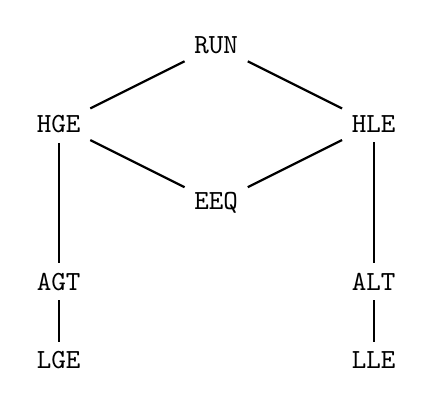
\begin{tikzpicture}[scale=2,baseline=(current bounding box.north)]
    \node (RUN) at (0,2.5) {\verb`RUN`};
    \node (HLE) at (1,2)  {\verb`HLE`};
    \node (HGE) at (-1,2) {\verb`HGE`};
    \node (ALT) at (1,1.0)  {\verb`ALT`};
    \node (EEQ) at (0,1.5) {\verb`EEQ`};
    \node (AGT) at (-1,1.0) {\verb`AGT`};
    \node (LLE) at (1,0.5)  {\verb`LLE`};
    \node (LGE) at (-1,0.5) {\verb`LGE`};

    \draw [thick] (RUN) -- (HLE);
    \draw [thick] (RUN) -- (HGE);
    \draw [thick] (HLE) -- (ALT);
    \draw [thick] (HGE) -- (AGT);
    \draw [thick] (HLE) -- (EEQ);
    \draw [thick] (HGE) -- (EEQ);
    \draw [thick] (ALT) -- (LLE);
    \draw [thick] (AGT) -- (LGE);
\end{tikzpicture}\hfill\hfill
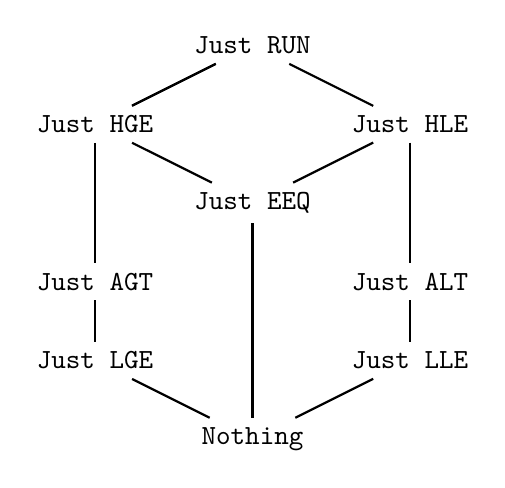
\begin{tikzpicture}[scale=2,baseline=(current bounding box.north)]
    \node (RUN) at (0,2.5) {\verb`Just RUN`};
    \node (HLE) at (1,2)  {\verb`Just HLE`};
    \node (HGE) at (-1,2) {\verb`Just HGE`};
    \node (ALT) at (1,1.0)  {\verb`Just ALT`};
    \node (EEQ) at (0,1.5) {\verb`Just EEQ`};
    \node (AGT) at (-1,1.0) {\verb`Just AGT`};
    \node (LLE) at (1,0.5)  {\verb`Just LLE`};
    \node (LGE) at (-1,0.5) {\verb`Just LGE`};
    \node (bot) at (0,0) {\verb`Nothing`};

    \draw [thick] (RUN) -- (HLE);
    \draw [thick] (RUN) -- (HGE);
    \draw [thick] (HLE) -- (ALT);
    \draw [thick] (HGE) -- (AGT);
    \draw [thick] (HLE) -- (EEQ);
    \draw [thick] (HGE) -- (EEQ);
    \draw [thick] (ALT) -- (LLE);
    \draw [thick] (AGT) -- (LGE);
    \draw [thick] (RUN) -- (HGE);
    \draw [thick] (bot) -- (LGE);
    \draw [thick] (bot) -- (LLE);
    \draw [thick] (bot) -- (EEQ);
\end{tikzpicture}\hfill\null

% max(4,u) LLE max(4,u+1)
% max(4,u) LLE max(6,u)

For the $\mathcal{L}$ normal form \verb`Tail`, the expressions are compared variablewise and these results are combined together with the semigroup operation.

For the $\mathcal{L}_{\ifop}$ normal form \verb`Const`, the expressions are compared for each relevant hypothetical and combined with the monoid operation.

\section{Solving Universe Levels}
\label{solv-uni-lvl}

As type inference progresses, more constraints are added to universe levels that need to be checked for consistency.
The actual state that is kept is a map from level expressions to level expressions, where each key-value pair represents the constraint that the key is \emph{greater than} the value.

\begin{verbatim}
newtype GESolver = GESolver (Map Const Const)
\end{verbatim}

The reason for this choice is that the conjuction of $u \ge v$ with $u \ge w$ is $u \ge \max(v, w)$. So having a single level expression for each upper bound suffices.

The primary aspect of solving is just saturating all of the known relations between expressions, starting with reflexivity.
For example, if $u \ge v$ is a constraint and $v \ge w$ is also a constraint, then $u \ge w$ is a constraint, by transitivity.
In practice, this means looking at all pairs of key-value pairs and adding $k_i \ge v_j$ when $v_i \ge k_j$.
However, this does not capture the distributivity of successor.
In general we want to adjust values by a constant that expresses when $k_j$ becomes less than $v_i$: for the largest $c \in \mathbb{Z}$ such that $v_i \ge k_j + c$, we instead add $k_i \ge v_j + c$ from the chain $k_i \ge v_i \ge k_j + c \ge v_j + c$.

If $k_i < v_i$ for some pair, then an error must be thrown since it is no longer consistent (this is important for termination of the saturation algorithm too).
In fact, more generally one wants to reduce the key if there are parts of $v_i$ that are strictly greater than the corresponding parts of $k_i$.
For example, if there is the constraint $\max(u, v) \ge \max(w, v+1)$, that is $\max(u, v) \ge w$ and $\max(u, v) \ge v+1$.
But the latter can only be satisfied by $u \ge v+1$, since $v \ngeq v+1$.
So $\max(u, v) = u$ and the constraint can be reduced to the pair $u \ge \max(w, v+1)$.

Finally there are a couple wrinkles to be figured out with $\imax$.
For example, if $\imax(u; v) > 0$ then $\imax(u; v) \ge \max(u, v)$, but recall that it is encoded in $\mathcal{L}_{\ifop}$ as $\max(\ifop(u; v), v)$.
As a more complicated situation with two variables, $\max(\imax(l; a), \imax(r; b)) > 0$ implies that $\max(a, b) > 0$ so $\max(\imax(l; a), \imax(r; b)) \ge \min(l, r)$, it would be weird to have to add a minimum operator, and again, it is not so obvious to see how this applies in the $\mathcal{L}_{\ifop}$ normal form in full generality and whether it does influence satisfiability.

However, by brute-force case analysis, it is possible to decide $\mathcal{L}_{\imax}$ in at worst exponential time over the plain $\mathcal{L}$ algorithm.

\iffalse
\begin{appdices}

\chapter{I Like Appendices}

\section{A Lovely Appendix}

\end{appdices}


\begin{bibliog}

\end{bibliog}
\fi

\end{document}

% end of file bardproj_template.tex
